% Pursuing Stacks (cotes 134-2 to 134-8): archive cote 134-3, site page 86 (PDF page 87), typescript page 86.
% typescript. Draft compared: ps2.tex:4486-4562.
% AI-transcribed by Claude Opus 5.5 (claude-opus-5-5, adaptive thinking, effort high), Message Batches API, batch ps1 (msgbatch_01Rv5hCaNTtUt4JHx1yqoHPL), 2026-11-12; image review recorded in records/CHECK_DECISIONS_134_3_4.tsv.
\scanpage{134-3/86}
\mspage{86}
including the customary ones for categories of simplices or cubes,  such as
\hand{\ensuremath{\Delta}}$^{f}$,\hand{\ensuremath{\Delta}},\hand{\ensuremath{\widetilde{\Delta}}}  and the cubical analogons.  If we admit the ``inspiring assumption''
that any autoequivalence of (Hot) is uniquely isomorphic to the identity
functor,  it will follow that the autoequivalence  (Hot)\hand{\ensuremath{\longrightarrow}}(Hot)  induced
by (11)  (where again i is any \inserted{weak} test functor)  is canonically isomorphic to
the identity.  This we checked directly (as part of the ``key result'' p.61
and following)  when we make on i the extra assumption that each category
i(a) has a final object.  In practical terms,  \uline{the role of a \inserted{weak} test functor}
\uline{i is to furnish us with a quasi-inverse of}
\[ W_{A}^{-1}A^{\hand{\wedge}} \hand{\ensuremath{\to}} W_{(\mathrm{Cat})}^{-1}(\mathrm{Cat}) = (\mathrm{Hot}) \]
\uline{induced by} $i_{A}$ ,  \uline{more handy than the one deduced from} $j_{A}$ \uline{by localization},
\uline{namely takin\hand{g}} $i^{*}$  \uline{instead of} $j_{A} = i_{A}^{*}$ .  In other terms,  for every homotopy
type,  described by an object C in (Cat),  we get a ready model in A\hand{\ensuremath{^{\wedge}}},  just
taking  $i^{*}(C) = (a\hand{\ensuremath{\mapsto}}\mathrm{Hom}(i(a),C))$.

In the theorem on p.61  just referred to,  one point was that we did
not assume beforehand that A was a weak test category,  but we were examining
two sets (a) and (b) of mutually equivalent conditions,  where  (a)  just
boils down to \inserted{$i_{A}i^{*}$} (11)  inducing an autoequivalence of (Hot),  while (b)
would be expressed (in the present terminology) by stating that \xout{moreover}
moreover A is a test category  (if we assume beforehand \unsure{\over[typed]{A}{i}}n  (b) that A is
aspheric)\hand{,} \inserted{plus a little more still on i.} It was not quite clear by then,  as it is now,  that this is
actually strictly stronger.  The somewhat bulky statement essentially redu-%
ces,  with the present background,  to the following
\uline{Proposition}   Let A be a small category,  i: A\hand{\ensuremath{\to}}(Cat)  a functor,  such
that for any  a in A,  i(a)  has a final object.  \deleted{Then} \inserted{Consider} the following condi-%
tions\hand{:}\deleted{are equivalent}:

(i)  A is a test category\hand{(}NB\xout{not} not only a weak one),  and i is a \inserted[typed]{weak} test
functor.

(ii)  T\over[typed]{H}{h}e element $i^{\hand{\ensuremath{*}}}(\hand{\ensuremath{\Delta}}_{1}\ )$ in A\hand{\ensuremath{^{\wedge}}} (namely  $a\hand{\ensuremath{\mapsto}}\mathrm{Crib}(i(a))$ is aspheric
over $e_{A^{\hand{\wedge}}}$  i.e. all products  $i^{*}(\hand{\ensuremath{\Delta}}_{1})\mathrm{x}a$  ($a$ \hand{\ensuremath{\in}} Ob A) are aspheric;
moreover $e_{A^{\hand{\wedge}}}$  is aspheric i.e.  \over{A}{A}  itself is aspheric.

(\over[typed]{i}{i}ii\over[typed]{)}{)}  There exists a homotopy interval  $(I,\hand{\ensuremath{\delta}}_{0},\hand{\ensuremath{\delta}}_{1})$ in A\hand{\ensuremath{^{\wedge}}}, and a map
in (Cat)  compatible with $\hand{\ensuremath{\delta}}_{0},\hand{\ensuremath{\delta}}_{1}$
\margin{(12)} \[ i_{\hand{!}}(I)\hand{\to}\hand{\ensuremath{\Delta}}_{1}\hand{,} \]
where $i_{\hand{!}}$ : A\hand{\ensuremath{^{\wedge}}}$\hand{\to}$(Cat)  is the canonical extension of i: A\hand{\ensuremath{\to}}(Cat)\hand{;}
\inserted{Moreover, A is aspheric.}
\margin{\diagram{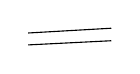
\begin{tikzpicture}[x=1em,y=1ex]\draw (0,0)--(3,.35);\draw (0,1)--(3,1.4);\end{tikzpicture}}}
The conditions  (ii)  and (iii) are equivalent and imply (i).

That (ii) implies (iii) is trivial by taking $I = i^{*}(\hand{\ensuremath{\Delta}}_{1})$ ;  the conver-%
se\hand{,} as we saw\hand{,} is a corollary of the comparison lemma for homotopy inter-%
vals  (p.60),  applied to  $I\hand{\ensuremath{\to}}i^{*}(\hand{\ensuremath{\Delta}}_{1}\ )$  corresponding to (12),  which is
